\documentclass[11pt]{paper}
\usepackage{palatino}
\usepackage{amsfonts,amsmath,amssymb}
% \usepackage{graphicx}

\usepackage{listings}
\usepackage{textcomp}
\usepackage{color}

\definecolor{dkgreen}{rgb}{0,0.6,0}
\definecolor{gray}{rgb}{0.5,0.5,0.5}
\definecolor{mauve}{rgb}{0.58,0,0.82}

\lstset{frame=tb,
  language=R,
  aboveskip=3mm,
  belowskip=3mm,
  showstringspaces=false,
  columns=flexible,
  basicstyle={\small\ttfamily},
  numbers=none,
  numberstyle=\tiny\color{gray},
  keywordstyle=\color{blue},
  commentstyle=\color{dkgreen},
  stringstyle=\color{mauve},
  breaklines=true,
  breakatwhitespace=true,
  tabsize=3
}



\ifx\pdftexversion\undefined
    \usepackage[dvips]{graphicx}
\else
    \usepackage[pdftex]{graphicx}
    \usepackage{epstopdf}
    \epstopdfsetup{suffix=}
\fi

\usepackage{subfig}


% This allows pdflatex to print the curly quotes in the
% significance codes in the output of the GAM.
\UseRawInputEncoding

\begin{document}

%%%%%%%%%%%%%%%%%%%%%%%%%%%%%%%%%%%%%%%%
% Problem Set 7
%%%%%%%%%%%%%%%%%%%%%%%%%%%%%%%%%%%%%%%%

\pagestyle{empty}
{\noindent\bf Spring 2021 \hfill Firstname M.~Lastname}
\vskip 16pt
\centerline{\bf University of Central Florida}
\centerline{\bf College of Business}
\vskip 16pt
\centerline{\bf QMB 6911}
\centerline{\bf Capstone Project in Business Analytics}
\vskip 10pt
\centerline{\bf Solutions:  Problem Set \#8}
\vskip 32pt
\noindent
% 
\section{Data Description}

This analysis follows the script \texttt{Tractor\_Reg\_Model.R} to produce a more accurate model for used tractor prices with the data from \texttt{TRACTOR7.csv} in the \texttt{Data} folder. 
The dataset includes the following variables.
\begin{table}[h!]
\begin{tabular}{l l l}

$saleprice_i$ & = & the price paid for tractor $i$ in dollars \\
% 
$horsepower_i$ & = & the horsepower of tractor $i$ \\
$age_i$ & = & the number of years since tractor $i$ was manufactured  \\
$enghours_i$ & = & the number of hours of use recorded for tractor $i$  \\
$diesel_i$ & = & an indicator of whether tractor $i$ runs on diesel fuel \\ %, $0$ otherwise \\
$fwd_i$ & = & an indicator of whether tractor $i$ has four-wheel drive \\ %, $0$ otherwise \\
$manual_i$ & = & an indicator of whether tractor $i$ has a manual transmission \\ %, $0$ otherwise \\
$johndeere_i$ & = & an indicator of whether tractor $i$ is manufactured by John Deere \\ %, $0$ otherwise \\
$cab_i$ & = & an indicator of whether tractor $i$ has an enclosed cab \\ %, $0$ otherwise \\
% 
$spring_i$ & = & an indicator of whether tractor $i$ was sold in April or May \\ %, $0$ otherwise \\
$summer_i$ & = & an indicator of whether tractor $i$ was sold between June and September \\ %, $0$ otherwise \\
$winter_i$ & = & an indicator of whether tractor $i$ was sold between December and March \\ %, $0$ otherwise \\

\end{tabular}
\end{table}
%

I will revisit the recommended linear model
from Problem Set \#7, 
which included a quadratic specification for horsepower.
This allowed for an increasing relationship 
between price and horsepower, 
for tractors with low horsepower, 
but a decreasing relationship for the tractors with high horsepower. 
I will investigate this nonlinear relationship
by incorporating a nonparametric specification
for the value of horsepower. 
Similarly, for the other continuous variables engine hours and age, 
to investigate whether these forms of depreciation
are best described with nonlinear forms. 


%%%%%%%%%%%%%%%%%%%%%%%%%%%%%%%%%%%%%%%%
\clearpage
\section{Linear Regression Model}
%%%%%%%%%%%%%%%%%%%%%%%%%%%%%%%%%%%%%%%%

A natural staring point is the recommended linear model
from Problem Set \#7. 

\subsection{Quadratic Specification for Horsepower}

Last week we considered the advice of
a used tractor dealer who reported that overpowered used tractors are hard to sell, since they consume more fuel. 
This implies that tractor prices often increase with horsepower, up to a point, but beyond that they decrease. 
To incorporate this advice, I created and included a variable for squared horsepower. 
A decreasing relationship for high values of horsepower
is characterized by 
a positive coefficient on the horsepower variable and
a negative coefficient on the squared horsepower variable. 

The results of this regression specification are shown in 
Table \ref{tab:reg_sq_horse}. 
% 
\input{../Tables/reg_sq_horse}
% 
The squared horsepower variable has a coefficient of $-2.081e-05$, which is nearly ten times as large as the standard error of $2.199e-06$, which is very strong evidence against the null hypothesis of a positive or zero coefficient. 
I conclude that the log of the sale price does decline for large values of horsepower. 


With the squared horsepower variable, the $\bar{R}^2$ is $0.764$, indicating that it is a much stronger model than the others we considered. 
The $F$-statistic is large, indicating that it is a better candidate than the simple average log sale price. 
The new squared horsepower variable is statistically significant and the theory behind it is sound, since above a certain point, added horsepower may not improve performance but will cost more to operate. 
This new model is much improved over the previous models with a linear specification for horsepower.
Next, I will attempt to improve on this specification. 





%%%%%%%%%%%%%%%%%%%%%%%%%%%%%%%%%%%%%%%%
\clearpage
\section{Nonlinear Specifications}
%%%%%%%%%%%%%%%%%%%%%%%%%%%%%%%%%%%%%%%%


% \clearpage
\subsection{Nonparametric Specification for Horsepower}


The specification in 
Table \ref{tab:reg_sq_horse}
assumes a quadratic functional form for
the relationship between price and horsepower. 
To consider the horsepower variable alone, 
while accounting for the effects of other variables, 
one can fit a nonparametric model to the residuals 
from a model of tractor prices, 
after regressing tractor prices on the other variables. 
This leaves only the variation in tractor prices that is not explained by the other variables. 
Going one step further, perform the same transformation to the horsepower variable:
take the residuals from a model of horsepower, 
after regressing horsepower on the other variables. 
This allows a model that would fit exactly the same as if it were estimated within a full model with all variables included. 

The models shown in
Table \ref{tab:reg_sq_horse_fwl}
illustrate this possibility. 
Model 1 is the original model in 
Table \ref{tab:reg_sq_horse}. 
Model 2 is a regression omitting the horsepower variables. 
Model 3 is a regression to predict horsepower with the other explanatory variables in Model 2.
Finally, Model 4 shows the coefficients for horsepower
from a regression of the residuals of Model 2
on the residuals from Model 3. 
Notice that these coefficients match those in Model 1. 
You might notice a slight difference in the standard errors, however, 
because these are calculated assuming coefficients 
for two variables, horsepower and squared horsepower,
rather than the full suite of ten parameters.
This equivalence of the coefficients can be used to fit
nonlinear models between a pair of variables by 
partialing out the effect of the other variables, 
using a mathematical result called the Frisch-Waugh-Lovell (FWL) theorem, 
maned after early statisticians and econometricians who used these methods. 

\input{../Tables/reg_sq_horse_fwl}

\pagebreak 
To illustrate the fit of the model, 
Figure \ref{fig:dev_vs_horse} shows a scatter plot 
of the residual log prices on horsepower. 
The observations are shown in blue
and the fitted values are shown in red.
The variation in the fitted values results from the 
fact that it is not plotted against the transformed excess horsepower variable used in the regressions.
Still, the quadratic pattern is apparent
and appears to match the data. 

\begin{figure}[h!]
  \centering
  \includegraphics[scale = 0.5, keepaspectratio=true]{../Figures/dev_vs_horse}
  \caption{Linear-Quadratic Model for Tractor Prices} \label{fig:dev_vs_horse}
\end{figure}



\pagebreak
As a comparison, Figure \ref{fig:dev_vs_horse_dev} 
augments the above by showing the plot against the 
residuals from the regression for horsepower:
the ``excess horsepower'' compared to what would be 
expected given the other characteristics of a tractor. 
The quadratic function is more clear from this perspective. 
This time, the variation in the fitted values results from the 
two-dimensional nature of the horsepower variable
when we consider the quadratic form.


\begin{figure}[h!]
  \centering
  \includegraphics[scale = 0.5, keepaspectratio=true]{../Figures/dev_vs_horse_dev}
  \caption{Linear-Quadratic Model for Tractor Prices: Excess Horsepower} \label{fig:dev_vs_horse_dev}
\end{figure}

\clearpage
Now consider a nonparametric specification for 
the relationship between prices and horsepower.
Figure \ref{fig:dev_np_vs_horse_dev} 
overlays the nonparametric estimate (shown in green) with the above in 
Figure \ref{fig:dev_vs_horse_dev}.
The pattern has more variation in slope but 
closely follows the prediction from the quadratic model. 
So far, it appears that the quadratic form
is close enough.

\begin{figure}[h!]
  \centering
  \includegraphics[scale = 0.5, keepaspectratio=true]{../Figures/dev_np_vs_horse_dev}
  \caption{Nonparametric Model for Tractor Prices: Excess Horsepower} \label{fig:dev_np_vs_horse_dev}
\end{figure}

 

\clearpage
Finally, consider a set of nonparametric specifications for 
the relationship between prices and horsepower.
Figure \ref{fig:dev_np_vs_horse_dev_bw} 
overlays other nonparametric estimates with the above in 
Figure \ref{fig:dev_np_vs_horse_dev}.
The points in orange and in magenta represent
alternate models with different degrees of smoothing. 
%
When we estimated probability densities,
we adjusted the bandwidth parameter to fit
with different degrees of smoothness.
The \texttt{loess} method used for the nonparametric method has a span parameter for this function.
The default smoother \texttt{span} (bandwidth parameter) is 0.75.

In the magenta points, with \texttt{span} parameter 0.1, the pattern has more variation in slope but 
closely follows the prediction from the quadratic model. 
The smoother curve in orange 
even more closely represents a quadratic line. 
Again, it appears that the quadratic form
is close enough.
Perhaps the result will be different for other continuous variables in the model.

\begin{figure}[h!]
  \centering
  \includegraphics[scale = 0.5, keepaspectratio=true]{../Figures/dev_np_vs_horse_dev_bw}
  \caption{Nonparametric Model for Tractor Prices: Excess Horsepower} \label{fig:dev_np_vs_horse_dev_bw}
\end{figure}





\clearpage
\subsection{Nonparametric Specification for Age}

As above, first conduct FWL regressions 
to reduce the problem to two dimensions. 
The models shown in
Table \ref{tab:reg_age_fwl}
illustrate this possibility. 
Model 1 is the same original model in 
Table \ref{tab:reg_sq_horse}. 
Model 2 is a regression omitting the age variable. 
Model 3 is a regression to predict age with the other explanatory variables in Model 2.
Finally, Model 4 shows the coefficient for age
from a regression of the residuals of Model 2
on the residuals from Model 3. 
Notice that these coefficients match those in Model 1. 


\begin{table}
\begin{center}
\begin{tabular}{l c c c c}
\hline
 & Model 1 & Model 2 & Model 3 & Model 4 \\
\hline
(Intercept)      & $1.55532^{***}$  & $1.55349^{***}$  & $0.58223^{***}$  &                \\
                 & $(0.01457)$      & $(0.01455)$      & $(0.09659)$      &                \\
squared\_mileage & $0.00000^{***}$  & $0.00000^{***}$  & $-0.00000^{***}$ &                \\
                 & $(0.00000)$      & $(0.00000)$      & $(0.00000)$      &                \\
make2            & $0.00842$        & $0.00833$        & $0.03083$        &                \\
                 & $(0.00744)$      & $(0.00744)$      & $(0.04943)$      &                \\
make3            & $0.00969$        & $0.00937$        & $0.10224$        &                \\
                 & $(0.00799)$      & $(0.00799)$      & $(0.05306)$      &                \\
make4            & $0.00764$        & $0.00740$        & $0.07386$        &                \\
                 & $(0.00657)$      & $(0.00657)$      & $(0.04363)$      &                \\
make5            & $0.00826$        & $0.00812$        & $0.04149$        &                \\
                 & $(0.00690)$      & $(0.00690)$      & $(0.04584)$      &                \\
make6            & $-0.04529^{***}$ & $-0.04541^{***}$ & $0.03704$        &                \\
                 & $(0.00670)$      & $(0.00670)$      & $(0.04452)$      &                \\
make7            & $-0.03770^{***}$ & $-0.03777^{***}$ & $0.02188$        &                \\
                 & $(0.00707)$      & $(0.00707)$      & $(0.04695)$      &                \\
make8            & $-0.07169^{***}$ & $-0.07128^{***}$ & $-0.12755$       &                \\
                 & $(0.00982)$      & $(0.00982)$      & $(0.06522)$      &                \\
make9            & $-0.06409^{***}$ & $-0.06368^{***}$ & $-0.13242$       &                \\
                 & $(0.01090)$      & $(0.01090)$      & $(0.07241)$      &                \\
damage2          & $-0.11601^{***}$ & $-0.11613^{***}$ & $0.03807$        &                \\
                 & $(0.01183)$      & $(0.01183)$      & $(0.07856)$      &                \\
damage3          & $-0.16372^{***}$ & $-0.16392^{***}$ & $0.06297$        &                \\
                 & $(0.01071)$      & $(0.01071)$      & $(0.07114)$      &                \\
damage4          & $-0.25179^{***}$ & $-0.25199^{***}$ & $0.06250$        &                \\
                 & $(0.01083)$      & $(0.01083)$      & $(0.07192)$      &                \\
damage5          & $-0.23679^{***}$ & $-0.23692^{***}$ & $0.04301$        &                \\
                 & $(0.01104)$      & $(0.01104)$      & $(0.07333)$      &                \\
damage6          & $-0.28664^{***}$ & $-0.28688^{***}$ & $0.07793$        &                \\
                 & $(0.01127)$      & $(0.01127)$      & $(0.07482)$      &                \\
damage7          & $-0.36724^{***}$ & $-0.36759^{***}$ & $0.11218$        &                \\
                 & $(0.01301)$      & $(0.01301)$      & $(0.08637)$      &                \\
damage8          & $-0.41161^{***}$ & $-0.41081^{***}$ & $-0.25535$       &                \\
                 & $(0.02113)$      & $(0.02113)$      & $(0.14031)$      &                \\
damage9          & $-0.39495^{***}$ & $-0.39599^{***}$ & $0.32838$        &                \\
                 & $(0.02595)$      & $(0.02595)$      & $(0.17233)$      &                \\
damage10         & $-0.44599^{***}$ & $-0.44649^{***}$ & $0.15937$        &                \\
                 & $(0.01535)$      & $(0.01535)$      & $(0.10193)$      &                \\
dealer2          & $-0.03791^{***}$ & $-0.03794^{***}$ & $0.01057$        &                \\
                 & $(0.00919)$      & $(0.00919)$      & $(0.06104)$      &                \\
dealer3          & $0.05242^{***}$  & $0.05129^{***}$  & $0.35918^{***}$  &                \\
                 & $(0.00693)$      & $(0.00691)$      & $(0.04590)$      &                \\
dealer4          & $-0.05643^{***}$ & $-0.05600^{***}$ & $-0.13649^{**}$  &                \\
                 & $(0.00637)$      & $(0.00636)$      & $(0.04226)$      &                \\
dealer5          & $0.03791^{***}$  & $0.03747^{***}$  & $0.13987^{*}$    &                \\
                 & $(0.00874)$      & $(0.00874)$      & $(0.05803)$      &                \\
dealer6          & $0.00365$        & $0.00345$        & $0.06191$        &                \\
                 & $(0.00621)$      & $(0.00621)$      & $(0.04126)$      &                \\
dealer7          & $0.03135^{***}$  & $0.03060^{***}$  & $0.23907^{***}$  &                \\
                 & $(0.00746)$      & $(0.00745)$      & $(0.04947)$      &                \\
dealer8          & $-0.05479^{***}$ & $-0.05457^{***}$ & $-0.06745$       &                \\
                 & $(0.00614)$      & $(0.00614)$      & $(0.04076)$      &                \\
dealer9          & $-0.06341^{***}$ & $-0.06304^{***}$ & $-0.11900^{*}$   &                \\
                 & $(0.00902)$      & $(0.00902)$      & $(0.05987)$      &                \\
mileage          & $-0.00000^{***}$ & $-0.00000^{***}$ & $0.00008^{***}$  &                \\
                 & $(0.00000)$      & $(0.00000)$      & $(0.00000)$      &                \\
age              & $-0.00314^{*}$   &                  &                  &                \\
                 & $(0.00135)$      &                  &                  &                \\
type1            & $0.10347^{***}$  & $0.10348^{***}$  & $-0.00034$       &                \\
                 & $(0.00359)$      & $(0.00359)$      & $(0.02387)$      &                \\
age\_resid       &                  &                  &                  & $-0.00314^{*}$ \\
                 &                  &                  &                  & $(0.00135)$    \\
\hline
R$^2$            & $0.23248$        & $0.23215$        & $0.83054$        & $0.00044$      \\
Adj. R$^2$       & $0.23070$        & $0.23042$        & $0.83016$        & $0.00036$      \\
Num. obs.        & $12492$          & $12492$          & $12492$          & $12492$        \\
\hline
\multicolumn{5}{l}{\scriptsize{$^{***}p<0.001$; $^{**}p<0.01$; $^{*}p<0.05$}}
\end{tabular}
\caption{Linear Model for Age: FWL Regressions}
\label{tab:reg_age_fwl}
\end{center}
\end{table}


\pagebreak 
To illustrate the fit of the model, 
Figure \ref{fig:dev_vs_age} shows a scatter plot 
of the residual log prices on age. 
The observations are shown in blue
and the fitted values are shown in red.
The variation in the fitted values results from the 
fact that it is not plotted against the transformed excess age variable used in the regressions.
Still, the linear pattern is apparent
and appears to match the data. 

\begin{figure}[h!]
  \centering
  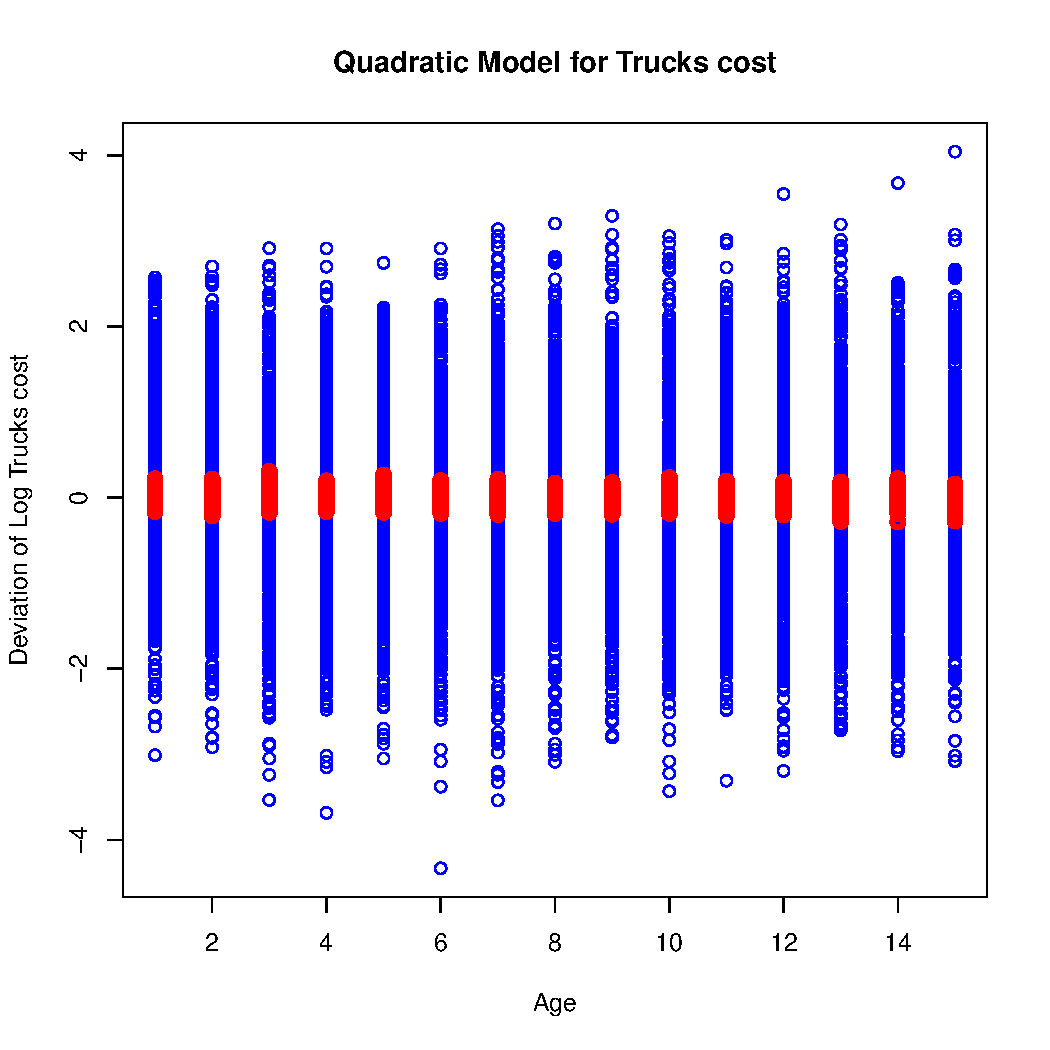
\includegraphics[scale = 0.5, keepaspectratio=true]{../Figures/dev_vs_age}
  \caption{Linear-Quadratic Model for Tractor Prices} \label{fig:dev_vs_age}
\end{figure}



\pagebreak
As a comparison, Figure \ref{fig:dev_vs_age_dev} 
augments the above by showing the plot against the 
residuals from the regression for age:
the ``excess age'' of a tractor compared to what would be 
expected given the other characteristics of the tractor. 
Notice that this time the fit follows a straight line,
since we have a single variable with no
quadratic transformation.

\begin{figure}[h!]
  \centering
  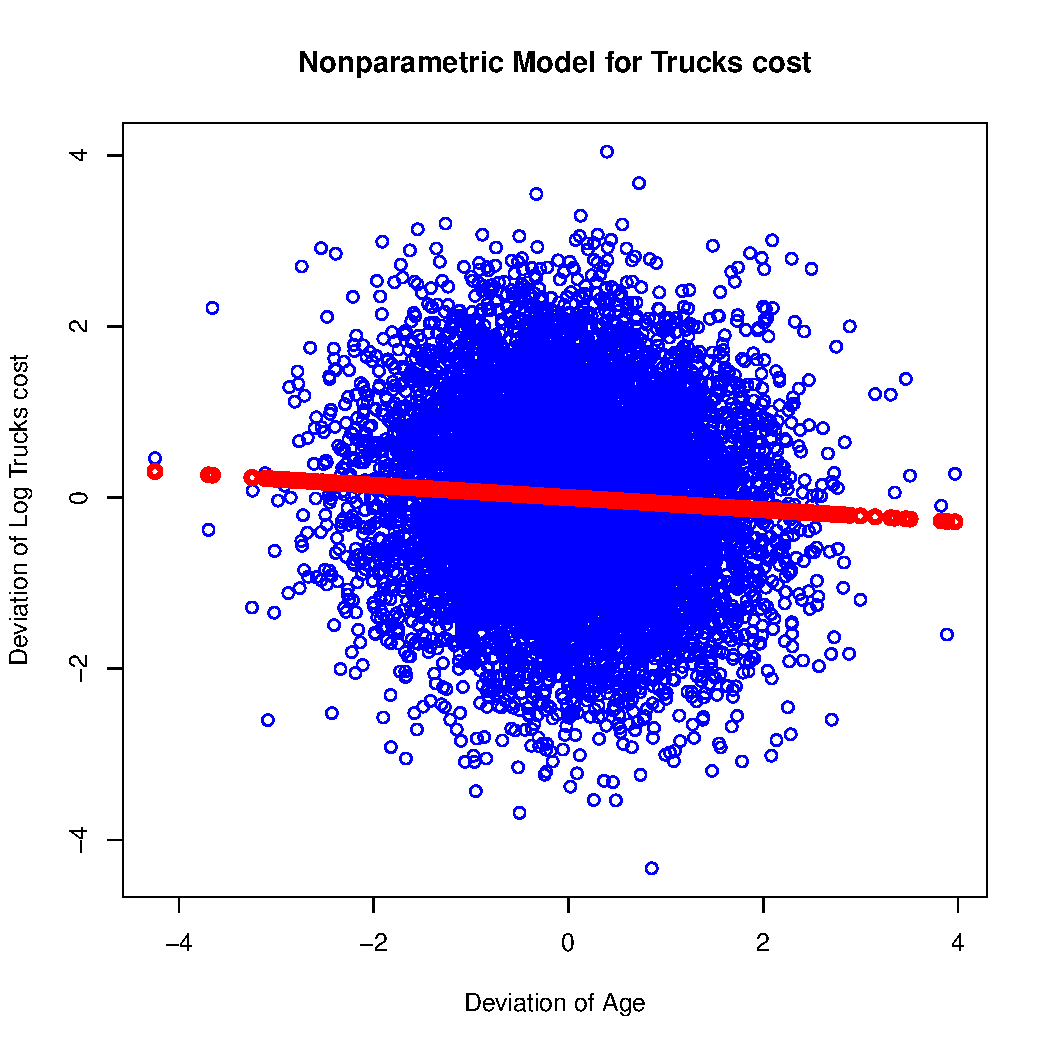
\includegraphics[scale = 0.5, keepaspectratio=true]{../Figures/dev_vs_age_dev}
  \caption{Linear-Quadratic Model for Tractor Prices: Excess Age} \label{fig:dev_vs_age_dev}
\end{figure}

\clearpage
Now consider a nonparametric specification for 
the relationship between prices and age.
Figure \ref{fig:dev_np_vs_age_dev} 
overlays the nonparametric estimate (shown in green) with the above in 
Figure \ref{fig:dev_vs_age_dev}.
The pattern has more variation in slope but 
closely follows the prediction from the linear model. 
Although the nonparametric estimate varies around the linear estimate,
it appears that the linear form
is a close enough approximation without the added complexity.
Next, I will explore the remaining continuous variable.


\begin{figure}[h!]
  \centering
  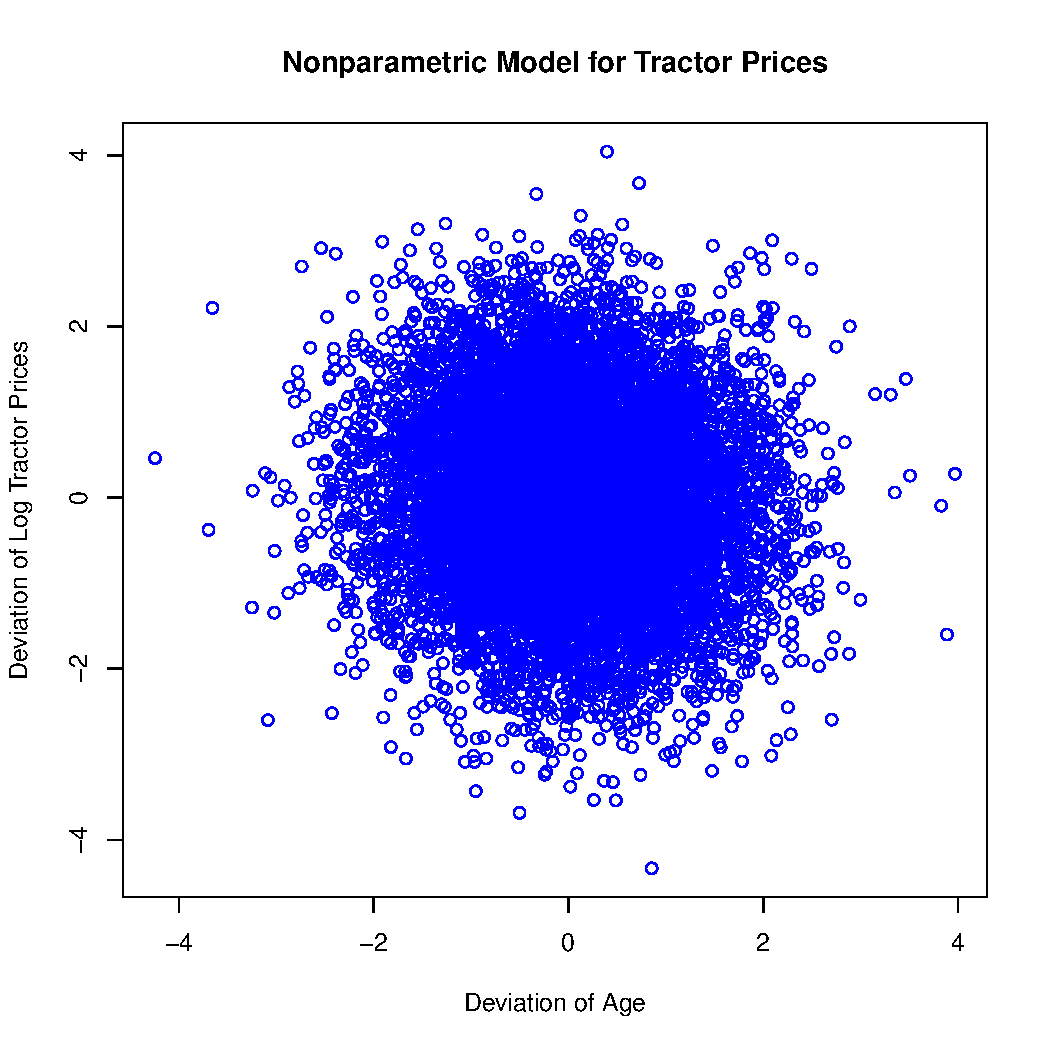
\includegraphics[scale = 0.5, keepaspectratio=true]{../Figures/dev_np_vs_age_dev}
  \caption{Nonparametric Model for Tractor Prices: Excess Age} \label{fig:dev_np_vs_age_dev}
\end{figure}





\clearpage
\subsection{Nonparametric Specification for Engine Hours}

As above, first conduct FWL regressions 
to reduce the problem to two dimensions. 
The models shown in
Table \ref{tab:reg_eng_fwl}
illustrate this possibility. 
Model 1 is the same original model in 
Table \ref{tab:reg_sq_horse}. 
Model 2 is a regression omitting the age variable. 
Model 3 is a regression to predict engine hours with the other explanatory variables in Model 2.
Finally, Model 4 shows the coefficient for engine hours
from a regression of the residuals of Model 2
on the residuals from Model 3. 
Notice that these coefficients match those in Model 1. 


\begin{table}
\begin{center}
\begin{tabular}{l c c c c}
\hline
 & Model 1 & Model 2 & Model 3 & Model 4 \\
\hline
(Intercept)      & $1.55532^{***}$  & $1.47603^{***}$  & $29418.40679^{***}$  &                 \\
                 & $(0.01457)$      & $(0.01351)$      & $(148.69894)$        &                 \\
squared\_mileage & $0.00000^{***}$  & $0.00000^{***}$  & $0.00000$            &                 \\
                 & $(0.00000)$      & $(0.00000)$      & $(0.00000)$          &                 \\
make2            & $0.00842$        & $0.01068$        & $71.80402$           &                 \\
                 & $(0.00744)$      & $(0.00761)$      & $(83.72605)$         &                 \\
make3            & $0.00969$        & $0.00925$        & $-11.60191$          &                 \\
                 & $(0.00799)$      & $(0.00817)$      & $(89.87057)$         &                 \\
make4            & $0.00764$        & $0.00356$        & $-145.40536^{*}$     &                 \\
                 & $(0.00657)$      & $(0.00671)$      & $(73.87609)$         &                 \\
make5            & $0.00826$        & $0.00882$        & $-20.89501$          &                 \\
                 & $(0.00690)$      & $(0.00706)$      & $(77.63335)$         &                 \\
make6            & $-0.04529^{***}$ & $-0.04461^{***}$ & $13.72200$           &                 \\
                 & $(0.00670)$      & $(0.00685)$      & $(75.39303)$         &                 \\
make7            & $-0.03770^{***}$ & $-0.03778^{***}$ & $-58.08645$          &                 \\
                 & $(0.00707)$      & $(0.00723)$      & $(79.52741)$         &                 \\
make8            & $-0.07169^{***}$ & $-0.06443^{***}$ & $126.87745$          &                 \\
                 & $(0.00982)$      & $(0.01004)$      & $(110.43065)$        &                 \\
make9            & $-0.06409^{***}$ & $-0.05468^{***}$ & $236.21408$          &                 \\
                 & $(0.01090)$      & $(0.01114)$      & $(122.57783)$        &                 \\
damage2          & $-0.11601^{***}$ & $-0.10590^{***}$ & $-8788.19435^{***}$  &                 \\
                 & $(0.01183)$      & $(0.01207)$      & $(132.78647)$        &                 \\
damage3          & $-0.16372^{***}$ & $-0.13549^{***}$ & $-11418.37114^{***}$ &                 \\
                 & $(0.01071)$      & $(0.01085)$      & $(119.39299)$        &                 \\
damage4          & $-0.25179^{***}$ & $-0.21916^{***}$ & $-17796.90557^{***}$ &                 \\
                 & $(0.01083)$      & $(0.01095)$      & $(120.46035)$        &                 \\
damage5          & $-0.23679^{***}$ & $-0.20209^{***}$ & $-18226.39807^{***}$ &                 \\
                 & $(0.01104)$      & $(0.01116)$      & $(122.75120)$        &                 \\
damage6          & $-0.28664^{***}$ & $-0.24560^{***}$ & $-19894.63077^{***}$ &                 \\
                 & $(0.01127)$      & $(0.01134)$      & $(124.76534)$        &                 \\
damage7          & $-0.36724^{***}$ & $-0.31054^{***}$ & $-24251.95014^{***}$ &                 \\
                 & $(0.01301)$      & $(0.01304)$      & $(143.53822)$        &                 \\
damage8          & $-0.41161^{***}$ & $-0.35430^{***}$ & $-26927.22915^{***}$ &                 \\
                 & $(0.02113)$      & $(0.02144)$      & $(235.96530)$        &                 \\
damage9          & $-0.39495^{***}$ & $-0.34019^{***}$ & $-27357.63751^{***}$ &                 \\
                 & $(0.02595)$      & $(0.02641)$      & $(290.65108)$        &                 \\
damage10         & $-0.44599^{***}$ & $-0.38397^{***}$ & $-27640.64177^{***}$ &                 \\
                 & $(0.01535)$      & $(0.01545)$      & $(169.98484)$        &                 \\
dealer2          & $-0.03791^{***}$ &                  &                      &                 \\
                 & $(0.00919)$      &                  &                      &                 \\
dealer3          & $0.05242^{***}$  &                  &                      &                 \\
                 & $(0.00693)$      &                  &                      &                 \\
dealer4          & $-0.05643^{***}$ &                  &                      &                 \\
                 & $(0.00637)$      &                  &                      &                 \\
dealer5          & $0.03791^{***}$  &                  &                      &                 \\
                 & $(0.00874)$      &                  &                      &                 \\
dealer6          & $0.00365$        &                  &                      &                 \\
                 & $(0.00621)$      &                  &                      &                 \\
dealer7          & $0.03135^{***}$  &                  &                      &                 \\
                 & $(0.00746)$      &                  &                      &                 \\
dealer8          & $-0.05479^{***}$ &                  &                      &                 \\
                 & $(0.00614)$      &                  &                      &                 \\
dealer9          & $-0.06341^{***}$ &                  &                      &                 \\
                 & $(0.00902)$      &                  &                      &                 \\
mileage          & $-0.00000^{***}$ & $-0.00000^{***}$ & $-0.00089$           &                 \\
                 & $(0.00000)$      & $(0.00000)$      & $(0.00223)$          &                 \\
age              & $-0.00314^{*}$   & $0.00059$        & $-37.71060^{*}$      &                 \\
                 & $(0.00135)$      & $(0.00137)$      & $(15.05526)$         &                 \\
type1            & $0.10347^{***}$  & $0.09734^{***}$  & $-420.02652^{***}$   &                 \\
                 & $(0.00359)$      & $(0.00365)$      & $(40.14198)$         &                 \\
cost\_resid      &                  &                  &                      & $0.00002^{***}$ \\
                 &                  &                  &                      & $(0.00000)$     \\
\hline
R$^2$            & $0.23248$        & $0.19718$        & $0.88633$            & $0.05760$       \\
Adj. R$^2$       & $0.23070$        & $0.19582$        & $0.88614$            & $0.05753$       \\
Num. obs.        & $12492$          & $12492$          & $12492$              & $12492$         \\
\hline
\multicolumn{5}{l}{\scriptsize{$^{***}p<0.001$; $^{**}p<0.01$; $^{*}p<0.05$}}
\end{tabular}
\caption{Linear Model for type : FWL Regressions}
\label{tab:reg_eng_fwl}
\end{center}
\end{table}


\pagebreak 
To illustrate the fit of the model, 
Figure \ref{fig:dev_vs_eng} shows a scatter plot 
of the residual log prices on engine hours. 
The observations are shown in blue
and the fitted values are shown in red.
The variation in the fitted values results from the 
fact that it is not plotted against the transformed excess engine hours variable used in the regressions.
Still, the linear pattern is apparent
and appears to match the data. 

\begin{figure}[h!]
  \centering
  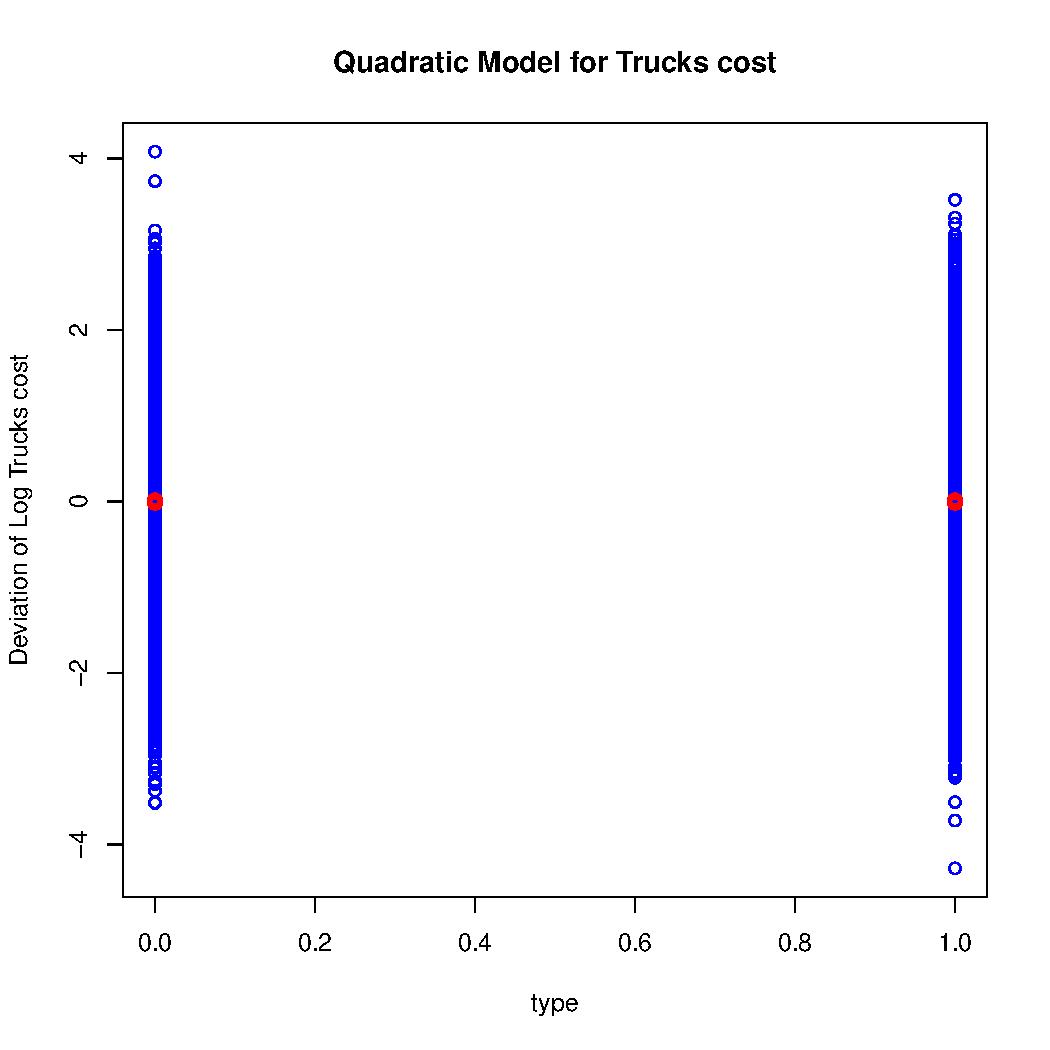
\includegraphics[scale = 0.5, keepaspectratio=true]{../Figures/dev_vs_eng}
  \caption{Linear-Quadratic Model for Tractor Prices} \label{fig:dev_vs_eng}
\end{figure}



\pagebreak
As a comparison, Figure \ref{fig:dev_np_vs_eng_dev} 
augments the above by showing the plot against the 
residuals from the regression for engine hours:
the ``excess engine hours'' of a tractor compared to what would be 
expected given the other characteristics of the tractor. 
As with age, the fit follows a straight line,
since we have a single variable with no
quadratic transformation.
% 
I move directly to the nonparametric specification for 
the relationship between prices and engine hours.
Figure \ref{fig:dev_np_vs_eng_dev} 
overlays the nonparametric estimate, shown in green. 
The pattern has more variation in slope but 
closely follows the prediction from the linear model. 
Although the nonparametric estimate varies around the linear estimate,
it appears that the linear form
is also a close enough approximation, 
just as was found for the age variable.


\begin{figure}[h!]
  \centering
  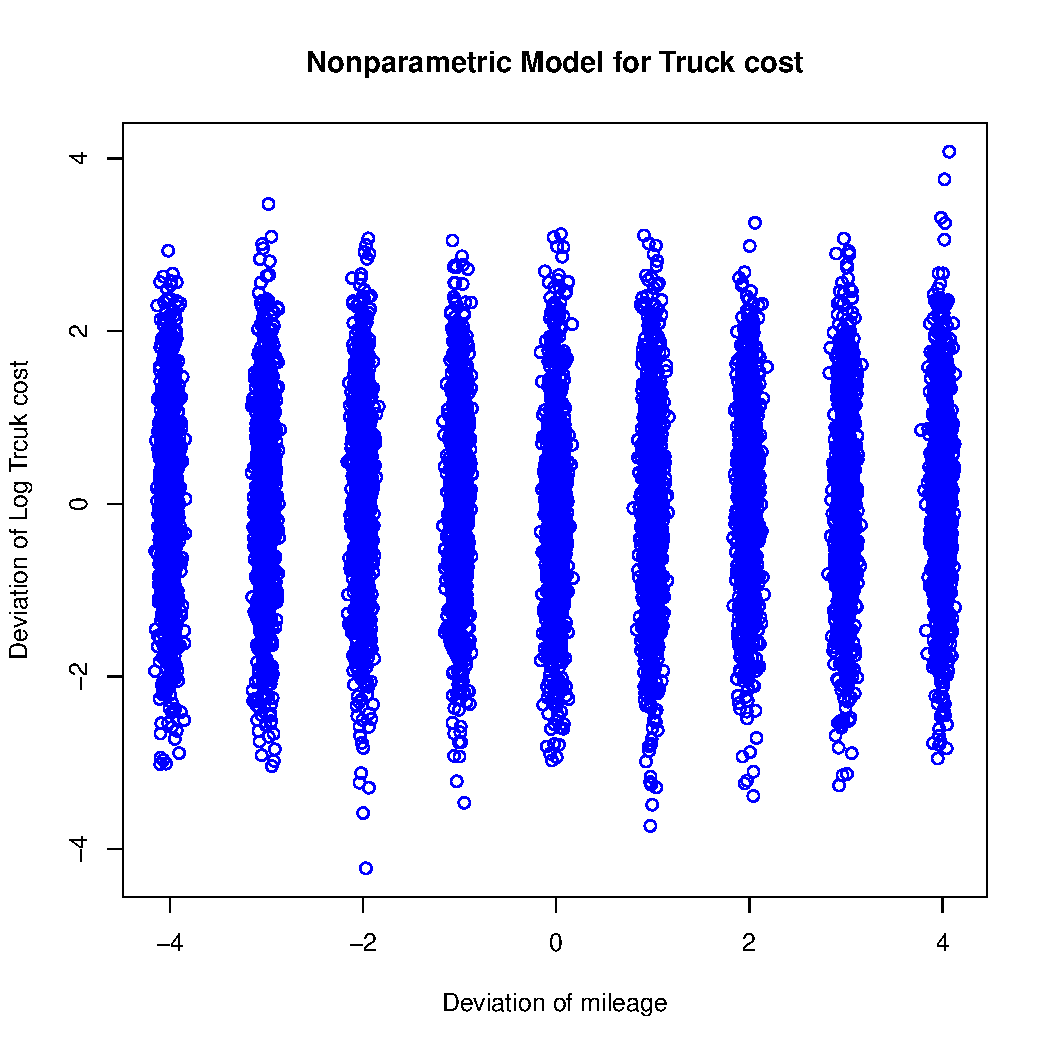
\includegraphics[scale = 0.5, keepaspectratio=true]{../Figures/dev_np_vs_eng_dev}
  \caption{Nonparametric Model for Tractor Prices: Excess Engine Hours} \label{fig:dev_np_vs_eng_dev}
\end{figure}

 

\pagebreak
\section{Semiparametric Estimates}

As I was building the above nonparametric models, 
I stored the predictions and will now use them as variables in 
linear models. 
Table \ref{tab:reg_semipar} 
shows the estimates from a set of models. 
Model 1 is the benchmark linear model in 
Table \ref{tab:reg_sq_horse}. 
Model 2 is a semi-parametric model
with a nonparametric fit on horsepower
substituted in for the horsepower variables.
Models 3 and 4 are semi-parametric models
with nonparametric fits on age and engine hours, respectively.
Model 5 is a maximally semiparametric model, 
with nonparametric fits for all continuous variables. 
For each of the single-variable semiparametric models, 
the coefficients are near one
and the fits are similar to the linear model. 
Even with maximal flexibility, the fit of Model 5
is not much better than the benchmark linear model. 
Across all models, the adjusted $\bar{R}^2$ values are all hovering around 0.80. 
All things considered, these are excellent models
and the linear model is sufficient.


\begin{table}
\begin{center}
\begin{tabular}{l c c c c c}
\hline
 & Model 1 & Model 2 & Model 3 & Model 4 & Model 5 \\
\hline
(Intercept)     & $8.76488^{***}$  & $8.65711^{***}$  & $8.95824^{***}$  & $8.76488^{***}$  & $8.74458^{***}$ \\
                & $(0.08135)$      & $(0.05515)$      & $(0.07530)$      & $(0.08135)$      & $(0.11028)$     \\
squared\_damage & $0.00459^{*}$    &                  & $0.00454^{*}$    & $0.00459^{*}$    &                 \\
                & $(0.00214)$      &                  & $(0.00213)$      & $(0.00214)$      &                 \\
make            & $-0.00619$       & $-0.00619$       & $-0.00580$       & $-0.00619$       & $-0.00587$      \\
                & $(0.00537)$      & $(0.00537)$      & $(0.00536)$      & $(0.00537)$      & $(0.00536)$     \\
damage          & $-0.04677$       & $-0.00394$       & $-0.05654^{*}$   & $-0.04677$       & $-0.01388$      \\
                & $(0.02543)$      & $(0.00808)$      & $(0.02536)$      & $(0.02543)$      & $(0.00873)$     \\
dealer          & $0.00196$        & $0.00232$        & $0.00245$        & $0.00196$        & $0.00270$       \\
                & $(0.00417)$      & $(0.00417)$      & $(0.00416)$      & $(0.00417)$      & $(0.00417)$     \\
mileage         & $-0.00001^{***}$ & $-0.00001^{***}$ & $-0.00001^{***}$ & $-0.00001^{***}$ & $-0.00001^{*}$  \\
                & $(0.00000)$      & $(0.00000)$      & $(0.00000)$      & $(0.00000)$      & $(0.00000)$     \\
age             & $-0.07163^{***}$ & $-0.06884^{***}$ &                  & $-0.07163^{***}$ & $-0.03239$      \\
                & $(0.01114)$      & $(0.01118)$      &                  & $(0.01114)$      & $(0.03528)$     \\
type            & $0.04438^{*}$    & $0.05465^{*}$    & $0.04512^{*}$    & $0.04438^{*}$    & $0.05433^{*}$   \\
                & $(0.02182)$      & $(0.02212)$      & $(0.02181)$      & $(0.02182)$      & $(0.02211)$     \\
damage\_np      &                  & $1.28304^{**}$   &                  &                  & $1.24683^{**}$  \\
                &                  & $(0.43922)$      &                  &                  & $(0.43894)$     \\
age\_np         &                  &                  & $1.01862^{***}$  &                  & $0.96938^{**}$  \\
                &                  &                  & $(0.13621)$      &                  & $(0.31910)$     \\
mileage\_np     &                  &                  &                  &                  & $0.69829$       \\
                &                  &                  &                  &                  & $(0.36384)$     \\
\hline
R$^2$           & $0.19087$        & $0.19119$        & $0.19206$        & $0.19087$        & $0.19269$       \\
Adj. R$^2$      & $0.19029$        & $0.19061$        & $0.19149$        & $0.19029$        & $0.19195$       \\
Num. obs.       & $9861$           & $9861$           & $9861$           & $9861$           & $9861$          \\
\hline
\multicolumn{6}{l}{\scriptsize{$^{***}p<0.001$; $^{**}p<0.01$; $^{*}p<0.05$}}
\end{tabular}
\caption{Semiparametric Models for Truck cost}
\label{tab:reg_semipar}
\end{center}
\end{table}






\pagebreak
\section{Generalized Additive Model}

\subsection{Linear Model}

As an example of the output from the GAM specification, 
I first estimated the model with no nonlinear terms, 
which is essentially a linear regression. 

\begin{verbatim}
Family: gaussian 
Link function: identity 

Formula:
log_cost ~ damage + squared_damage + age + make + damage + dealer + 
    mileage + age + type

Parametric coefficients:
                 Estimate Std. Error t value Pr(>|t|)    
(Intercept)     8.765e+00  8.135e-02 107.740  < 2e-16 ***
damage         -4.677e-02  2.543e-02  -1.839   0.0659 .  
squared_damage  4.595e-03  2.135e-03   2.152   0.0314 *  
age            -7.163e-02  1.114e-02  -6.430 1.34e-10 ***
make           -6.194e-03  5.368e-03  -1.154   0.2486    
dealer          1.964e-03  4.168e-03   0.471   0.6376    
mileage        -5.053e-06  1.062e-06  -4.756 2.01e-06 ***
type            4.438e-02  2.182e-02   2.034   0.0420 *  
---
Signif. codes:  0 �***� 0.001 �**� 0.01 �*� 0.05 �.� 0.1 � � 1


R-sq.(adj) =   0.19   Deviance explained = 19.1%
GCV = 1.1444  Scale est. = 1.1435    n = 9861
\end{verbatim}

\pagebreak
\subsection{Semiparametric Model}


Further investigating the results of the full semiparametric specification
in Model 5 of Table \ref{tab:reg_semipar},
I estimated the model with all three continuous variables specified as nonparametric functions. 
The result was that 
almost all the variables---both linear and nonlinear---were 
statistically significant. 
The only exception was a loss in significance of the diesel indicator. 


\begin{verbatim}
Family: gaussian 
Link function: identity 

Formula:
ror ~ s(mileage) + s(age)

Parametric coefficients:
            Estimate Std. Error t value Pr(>|t|)    
(Intercept) 1.191988   0.001692   704.4   <2e-16 ***
---
Signif. codes:  0 �***� 0.001 �**� 0.01 �*� 0.05 �.� 0.1 � � 1

Approximate significance of smooth terms:
             edf Ref.df      F p-value    
s(mileage) 6.059  7.350 20.651  <2e-16 ***
s(age)     8.705  8.946  2.036  0.0233 *  
---
Signif. codes:  0 �***� 0.001 �**� 0.01 �*� 0.05 �.� 0.1 � � 1

R-sq.(adj) =  0.0726   Deviance explained = 7.37%
GCV = 0.035816  Scale est. = 0.03577   n = 12492
\end{verbatim}

On the other hand, 
the adjusted R-squared has not increased very much, 
from 0.799 to 0.819 under this specification, 
which may not justify the added complexity of the model.
Perhaps more importantly, the coefficients on the 
linear terms are very similar across models, 
indicating that the models support similar conclusions relating to any business decision involving
the John Deere premium. 
With this second model, we have even more support for those conclusions
and are certain that the conclusions are not 
coincidental results of the
functional form decisions for previous models.


Perhaps as a middle ground, we can estimate a model with a 
nonparametric specification for the horsepower variable alone, 
since it seems to have a nonlinear relationship with value in either case. 
This retains most of the predictive value of the maximally 
semiparametric model and accommodates the 
nonlinear relationship with value of horsepower. 

\begin{verbatim}
Family: gaussian 
Link function: identity 

Formula:
log_cost ~ s(damage) + age + make + damage + dealer + mileage + 
    age + type

Parametric coefficients:
              Estimate Std. Error t value Pr(>|t|)    
(Intercept)  1.209e+00  3.007e-02  40.192  < 2e-16 ***
age         -7.148e-02  1.114e-02  -6.417 1.46e-10 ***
make        -6.227e-03  5.368e-03  -1.160   0.2461    
damage       1.310e+00  9.977e-03 131.253  < 2e-16 ***
dealer       1.870e-03  4.169e-03   0.448   0.6538    
mileage     -5.072e-06  1.062e-06  -4.774 1.84e-06 ***
type         4.453e-02  2.182e-02   2.041   0.0413 *  
---
Signif. codes:  0 �***� 0.001 �**� 0.01 �*� 0.05 �.� 0.1 � � 1

Approximate significance of smooth terms:
           edf Ref.df    F p-value    
s(damage) 4.75  5.914 3432  <2e-16 ***
---
Signif. codes:  0 �***� 0.001 �**� 0.01 �*� 0.05 �.� 0.1 � � 1

Rank: 15/16
R-sq.(adj) =  0.191   Deviance explained = 19.1%
GCV = 1.1444  Scale est. = 1.1431    n = 9861
\end{verbatim}



%%%%%%%%%%%%%%%%%%%%%%%%%%%%%%%%%%%%%%%%
\end{document}
%%%%%%%%%%%%%%%%%%%%%%%%%%%%%%%%%%%%%%%%
